\chapter{Pulse Speed} 
\lstset{style=6502Style}

\begin{figure}[H]
    \centering
    \begin{adjustbox}{width=10.5cm,margin=0cm}
      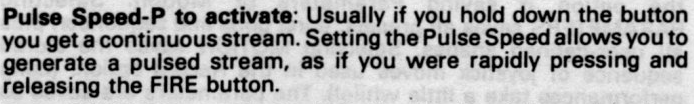
\includegraphics[width=12cm]{src/pulsespeed/pulsespeed.png}%
    \end{adjustbox}
    \caption{
      Excerpt from Manual (Part No. LC1982-Vb). Pulse Speed.
      }
\end{figure}

\begin{lstlisting}[caption=From \icode{CheckKeyboardInput}.]
MaybePPressed   
        CMP #KEY_P ; P pressed
        BNE MaybeHPressed

        ; P pressed.
        ; Pulse Speed P to activate: Usually if you hold down the button you
        ; get a continuous stream. Setting the Pulse Speed allows you to
        ; generate a pulsed stream, as if you were rapidly pressing and
        ; releasing the FIRE button.
        LDA #PULSE_SPEED
        STA currentVariableMode
        RTS 
\end{lstlisting}

\begin{figure}[H]
    \centering
    \begin{adjustbox}{width=3cm,margin=11cm -12cm}
      
\includegraphics[width=12cm]{src/pulsespeed/pulsespeed-low.png}%
    \end{adjustbox}
    \begin{adjustbox}{width=10.5cm,center}
      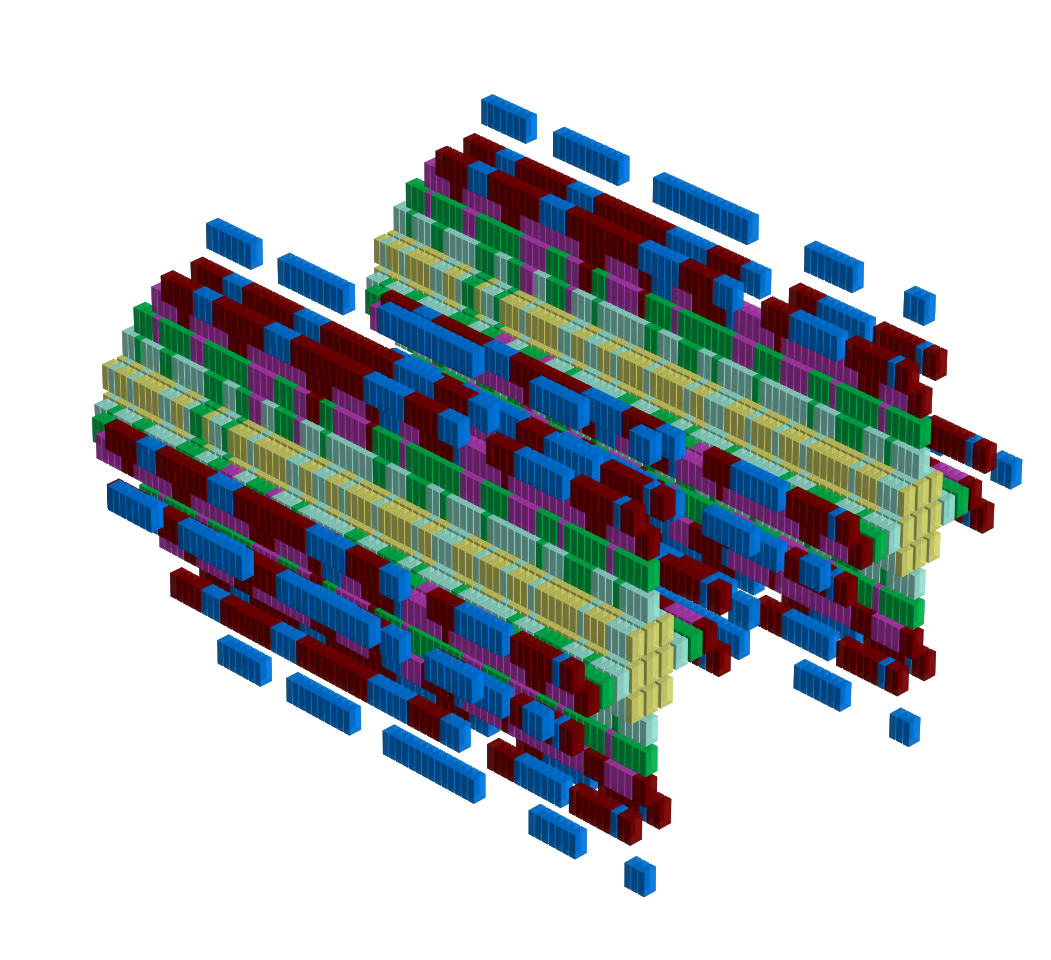
\includegraphics[width=12cm]{src/pulsespeed/pattern0-45.png}%
    \end{adjustbox}
    \begin{adjustbox}{width=3cm,margin=11cm -12cm}
      
\includegraphics[width=12cm]{src/pulsespeed/pulsespeed-high.png}%
    \end{adjustbox}
    \begin{adjustbox}{width=10.5cm,margin=0cm -2cm}
      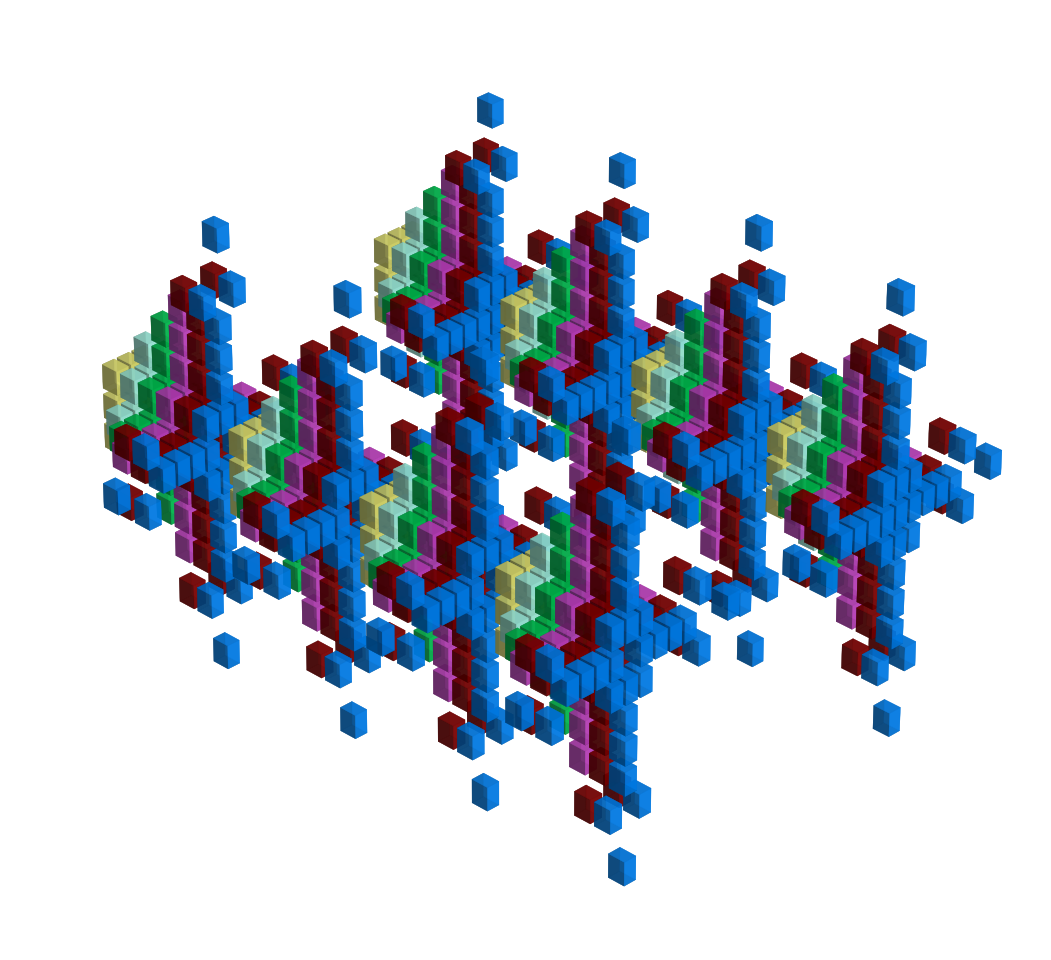
\includegraphics[width=12cm]{src/pulsespeed/pattern1-45.png}%
    \end{adjustbox}
    \caption{Effect of low and high values for Pulse Speed}
\end{figure}


\begin{lstlisting}[caption=From \icode{CheckKeyboardInputForActiveVariable}. Pressing the < and > keys increments and
decrements the value in presetValueArray pointed to by \icode{X}\, i.e. \icode{currentVariableMode}.]
UpdateVariableDisplay   
        LDA #>SCREEN_RAM + $03D0
        STA colorBarColorRamHiPtr
        LDA #<SCREEN_RAM + $03D0
        STA colorBarColorRamLoPtr

        LDX currentVariableMode
        LDA lastKeyPressed
        CMP #$2C ; > pressed?
        BNE MaybeLeftArrowPressed

        ; > pressed, increase the value bar and write
        ; it to the approiate place in presetValueArray
        INC presetValueArray,X
        LDA presetValueArray,X
        ; Make sure we don't exceed the max value.
        CMP maxValueForPresetValueArray,X
        BNE MaybeInColorMode
        DEC presetValueArray,X
        JMP MaybeInColorMode
\end{lstlisting}

\begin{lstlisting}[caption=From \icode{ActivateSequencer}.]
; This is where the presets get loaded to. It represents
; the data structure for the presets.
; currentVariableMode is an index into this data structure
; when the user adjusts settings.
presetValueArray
unusedPresetByte        .BYTE $00
smoothingDelay          .BYTE $0C
cursorSpeed             .BYTE $02
bufferLength            .BYTE $1F
pulseSpeed              .BYTE $01; <-- Pulse Speed is here at position \icode{\$04}.
indexForColorBarDisplay .BYTE $01
lineWidth               .BYTE $07
sequencerSpeed          .BYTE $04 
pulseWidth              .BYTE $01
baseLevel               .BYTE $07
presetColorValuesArray  .BYTE BLACK,BLUE,RED,PURPLE,GREEN,CYAN,YELLOW,WHITE
trackingActivated       .BYTE $FF
lineModeActivated       .BYTE $00
presetIndex            .BYTE $05
\end{lstlisting}


\begin{lstlisting}[caption=From \icode{MainInterruptHandler}.]
DecrementPulseSpeedCounter   
        DEC currentPulseSpeedCounter
        BEQ RefreshPulseSpeed
        JMP DrawCursorAndReturnFromInterrupt
        ; Returns

RefreshPulseSpeed   
        LDA pulseSpeed
        STA currentPulseSpeedCounter
        LDA pulseWidth
        STA currentPulseWidth
\end{lstlisting}
